
\subsection{Vorticity – Wirbelstärke in der Atmosphäre}

Die grossräumige Bewegung der Luft in der Atmosphäre lässt sich nicht nur durch die
Geschwindigkeit beschreiben, sondern auch durch ihre Rotationseigenschaften.
Diese Eigenschaft wird durch die sogenannte \emph{Vorticity} (Wirbelstärke)
quantifiziert. Physikalisch beschreibt sie die Tendenz eines Luftpakets, sich
um seine eigene vertikale Achse zu drehen.

Mathematisch ist die Vorticity definiert als Rotation des
Geschwindigkeitsfeldes:
\begin{equation}
	\vec{\zeta} = \nabla \times \vec{u}.
	\label{rossby:eq:vorticity}
\end{equation}
Für grossräumige Strömungen in der Atmosphäre betrachtet man hauptsächlich die vertikale Komponente dieser Rotation, die sogenannte \emph{relative Vorticity}.
In kartesischen Koordinaten ergibt sich diese im einfachsten Fall zu:
\begin{equation}
	\zeta = \frac{\partial v}{\partial x} - \frac{\partial u}{\partial y},
	\label{rossby:eq:relative_vorticity}
\end{equation}
wobei \(u\) und \(v\) die zonale bzw. meridionale Windkomponente bezeichnen.
Positive Vorticity (\(\zeta > 0\)) steht für eine zyklonale Rotation (auf der Nordhalbkugel gegen den Uhrzeigersinn), negative Vorticity (\(\zeta < 0\)) für eine antizyklonale Rotation (im Uhrzeigersinn).
\begin{figure}
	\centering
	% Erste Reihe
	\begin{minipage}{0.32\linewidth}
		\centering
		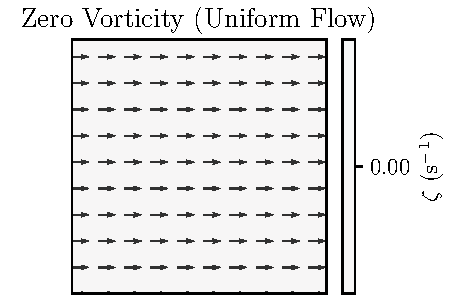
\includegraphics[width=\linewidth]{papers/rossby/images/vorticity_plot0.pdf}\\
		{\small \( \vec{u} = (2,0),\ \zeta = 0\)}
	\end{minipage}
	\begin{minipage}{0.32\linewidth}
		\centering
		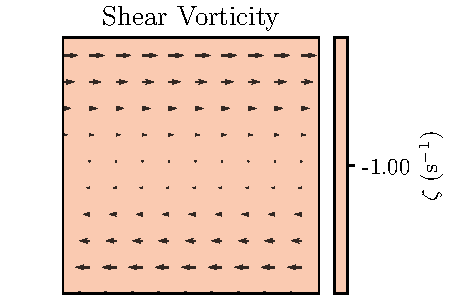
\includegraphics[width=\linewidth]{papers/rossby/images/vorticity_plot1.pdf}\\
		{\small \( \vec{u} = (y,0),\ \zeta = -1\)}
	\end{minipage}
	\begin{minipage}{0.32\linewidth}
		\centering
		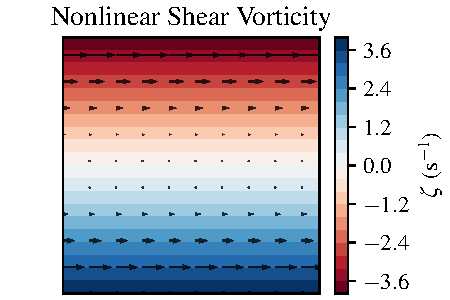
\includegraphics[width=\linewidth]{papers/rossby/images/vorticity_plot2.pdf}\\
		{\small \( \vec{u} = (y^2,0),\ \zeta = -2y\)}
	\end{minipage}
	\\[15pt]
	% Zweite Reihe
	\begin{minipage}{0.32\linewidth}
		\centering
		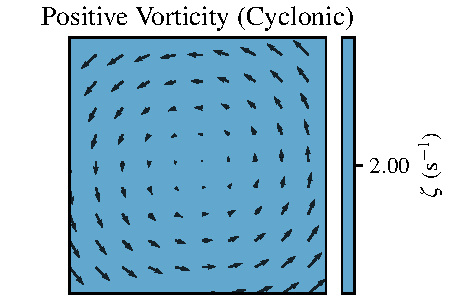
\includegraphics[width=\linewidth]{papers/rossby/images/vorticity_plot3.pdf}\\
		{\small \( \vec{u} = (-y,x),\ \zeta = 2\)}
	\end{minipage}
	\begin{minipage}{0.32\linewidth}
		\centering
		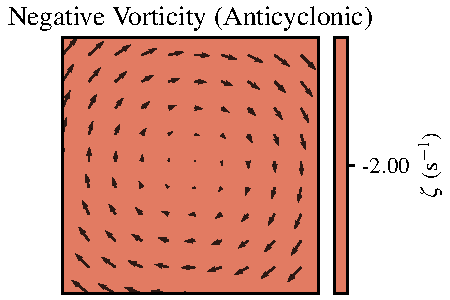
\includegraphics[width=\linewidth]{papers/rossby/images/vorticity_plot4.pdf}\\
		{\small \( \vec{u} = (y,-x),\ \zeta = -2\)}
	\end{minipage}

	\caption{Beispiele für verschiedene Vorticity-Fälle in idealisierten Strömungsfeldern.}
	\label{fig:vorticity_examples}
\end{figure}

\subsection{Absolute Vorticity}

Die bisher betrachtete relative Vorticity beschreibt die Rotation eines
Luftpakets relativ zum Erdboden. Da sich jedoch auch die Erde selbst dreht,
muss diese planetare Rotation bei der Beschreibung der Gesamtdrehung
berücksichtigt werden. Daraus ergibt sich der Begriff der \emph{absoluten
	Vorticity}, welche die Summe aus relativer und planetarer Vorticity darstellt.

Die planetare Vorticity wird durch den \emph{Coriolis-Parameter} \(
f = 2 \Omega \sin \varphi \) beschrieben, wobei \( \Omega \) die
Erdrotationsrate und \( \varphi \) die geographische Breite ist. Dieser
Ausdruck ergibt sich aus der Projektion der Erdrotation auf die lokale
Vertikale. Die absolute Vorticity ergibt sich somit zu:
\begin{equation}
	\eta = \zeta + f
	\label{rossby:eq:absolute_vorticity}
\end{equation}
wobei \( \zeta \) die relative und \( f \) die planetare Vorticity ist.

% Die absolute Vorticity ist eine Erhaltungsgrösse in der reibungsfreien, barotropen Atmosphäre, wenn keine vertikalen Bewegungen stattfinden.
% Sie spielt daher eine zentrale Rolle in der dynamischen Meteorologie und bildet die Grundlage für das Konzept der \emph{potenziellen Vorticity}, welches zusätzlich die Schichtung der Atmosphäre berücksichtigt.

\subsection{Potenzielle Vorticity und ihre Erhaltung}

Die \emph{potenzielle Vorticity} erweitert das Konzept der \emph{absoluten
Vorticity} um die vertikale Struktur der Atmosphäre. In ihrer Erhaltungsform
ist sie ein zentrales Werkzeug zur Beschreibung grossskaliger Strömungen und
Wellenprozesse.

Unter vereinfachten Bedingungen, barotrope, reibungsfreie Atmosphäre mit
konstantem Luftvolumen, lautet die Definition:
\begin{equation}
	q = \frac{\zeta + f}{H},
	\label{rossby:eq:potential_vorticity}
\end{equation}
wobei \(\zeta\) die relative Vorticity, \(f\) den Coriolis-Parameter und \(H\) die effektive Schichthöhe der betrachteten Luftsäule bezeichnet.
Dieser Ausdruck berücksichtigt sowohl die horizontale Rotation als auch die vertikale Ausdehnung eines Luftpakets. 

Man kann die potentielle Vorticity als die \emph{allgemeinere Erhaltungsgröße}
verstehen, welche die Drehimpulserhaltung als Spezialfall umfasst. Während
die Drehimpulserhaltung nur die axiale Rotation einer Luftsäule beschreibt,
fasst die potentielle Vorticity zusätzlich Effekte der vertikalen Schichtung
und der relativen Vorticity zusammen. Eine anschauliche Analogie ist die
Eiskunstläufer:in, die ihre Rotationsgeschwindigkeit ändert, wenn sie die Arme
an den Körper zieht oder ausstreckt: die Drehimpulserhaltung erzwingt eine
Anpassung der Rotationsgeschwindigkeit an die veränderte Trägheit. In der
Atmosphäre entspricht dies der Anpassung der Vorticity an Änderungen der
Schichthöhe, wie sie in Gl.~\eqref{rossby:eq:potential_vorticity} beschrieben ist.



\begin{figure}
	\centering
	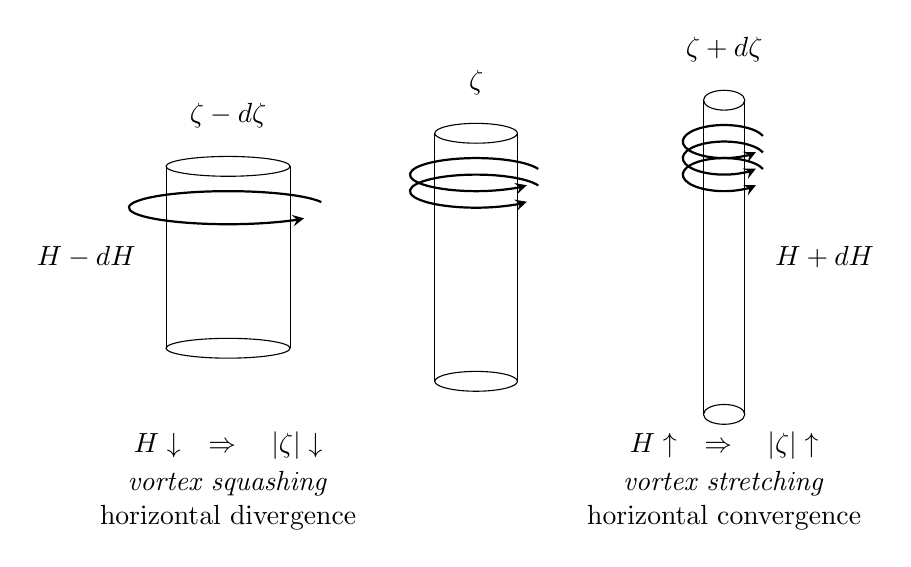
\begin{tikzpicture}[scale=1.05, >=stealth]
		% params
		\def\Rone{0.5}\def\Rtwo{0.25}\def\Rthree{0.75}\def\r{0.12}
		\def\H{3.0}  \def\dH{0.8}
		\def\DX{3}

		% guide rays (dashed perspective)
		% \draw[dashed] (-0.2,\H) -- (\DX+0.2,\H);
		% \draw[dashed] (-0.2,0)  -- (\DX+0.2,0);

		% center cylinder (height H)
		\draw (0,0) ellipse ({\Rone} and {\r});
		\draw (-\Rone,0) -- (-\Rone,\H);
		\draw (\Rone,0) -- (\Rone,\H);
		\draw (0,\H) ellipse ({\Rone} and {\r});
		\node[above] at (0,\H+0.35) {$\zeta$};
		% \draw[->] (1.4,1.7) -- (0.7,1.7);

		% right cylinder (H+dH)
		\begin{scope}[xshift=\DX cm]
			\draw (0,{-\dH/2}) ellipse ({\Rtwo} and {\r});         % bottom
			\draw (-\Rtwo,{-\dH/2}) -- (-\Rtwo,{\H+\dH/2});
			\draw ( \Rtwo,{-\dH/2}) -- ( \Rtwo,{\H+\dH/2});
			\draw (0,{\H+\dH/2}) ellipse ({\Rtwo} and {\r});        % top
			\node[above] at (0,{\H+\dH/2+0.35}) {$\zeta+d\zeta$};
			\node[right] at (\Rtwo+0.25,{\H/2}) {$H+dH$};  % center the label
			% \draw[->] (-1.4,{\H/2}) -- (-0.7,{\H/2});
		\end{scope}


		\begin{scope}[xshift={-\DX cm}]
			\draw (0,{ \dH/2}) ellipse ({\Rthree} and {\r});          % bottom
			\draw (-\Rthree,{ \dH/2}) -- (-\Rthree,{\H-\dH/2});
			\draw ( \Rthree,{ \dH/2}) -- ( \Rthree,{\H-\dH/2});
			\draw (0,{\H-\dH/2}) ellipse ({\Rthree} and {\r});        % top
			\node[above] at (0,{\H-\dH/2+0.35}) {$\zeta-d\zeta$};
			\node[left]  at (-\Rthree-0.25,{\H/2}) {$H-dH$}; % center the label
		\end{scope}
		% spin symbols on tops
		% spin symbols: use H±dH/2 so the midline matches
		% at the top (tweak to taste)
		\def\spinrxone{1.2}\def\spinrxtwo{0.8}\def\spinrxthree{0.5}
		\def\spinry{0.2}\def\spinstart{20}

		\foreach \x/\y/\spinrx in {-\DX/{\H-\dH/2}/\spinrxone, 0/{\H}/\spinrxtwo, \DX/{\H+\dH/2}/\spinrxthree}{
		\begin{scope}[xshift=\x cm]
			\draw[->, thick]
			({\spinrx*cos(\spinstart)}, {\y-0.5 + \spinry*sin(\spinstart)})
			arc[start angle=\spinstart, end angle=\spinstart+300,
					x radius=\spinrx, y radius=\spinry];
		\end{scope}
		}

		\foreach \x/\y/\spinrx in { 0/{\H}/\spinrxtwo, \DX/{\H+\dH/2}/\spinrxthree}{
		\begin{scope}[xshift=\x cm]
			\draw[->, thick]
			({\spinrx*cos(\spinstart)}, {\y-0.7 + \spinry*sin(\spinstart)})
			arc[start angle=\spinstart, end angle=\spinstart+300,
					x radius=\spinrx, y radius=\spinry];
		\end{scope}
		}

		\foreach \x/\y/\spinrx in { \DX/{\H+\dH/2}/\spinrxthree}{
		\begin{scope}[xshift=\x cm]
			\draw[->, thick]
			({\spinrx*cos(\spinstart)}, {\y-0.9 + \spinry*sin(\spinstart)})
			arc[start angle=\spinstart, end angle=\spinstart+300,
					x radius=\spinrx, y radius=\spinry];
		\end{scope}
		}

		% captions
		\node[align=center] at (-\DX,-1.2)
		{$H\downarrow \quad \Rightarrow \quad |\zeta|\downarrow$\\[2pt]\emph{vortex squashing}\\ horizontal divergence};
		\node[align=center] at (\DX,-1.2)
		{$H\uparrow \quad \Rightarrow \quad |\zeta|\uparrow$\\[2pt]\emph{vortex stretching}\\ horizontal convergence};
	\end{tikzpicture}


	\caption{%
		Schematische Darstellung der Erhaltung der potenziellen Vorticity.
		Die mittlere Luftsäule zeigt den Ausgangszustand mit Höhe $H$ und relativer
		Vorticity $\zeta$. Eine Verringerung der Säulenhöhe ($H \downarrow$) führt
		über horizontale Divergenz zu einer Abnahme von $|\zeta|$
		(\emph{vortex squashing}), während eine Vergrösserung ($H \uparrow$) über
		Konvergenz zu einer Zunahme von $|\zeta|$ (\emph{vortex stretching}) führt.
		Damit bleibt das Verhältnis $q=(\zeta+f)/H$ entlang der Trajektorie eines
		Luftpakets konstant (eigene Darstellung inspieriert durch \cite{rossby:beal_pv}).%
	}
	\label{fig:pv_conservation}
\end{figure}

Ein zentrales Ergebnis der quasi-geostrophischen Theorie ist die Erhaltung der
potenziellen Vorticity entlang der Trajektorie eines Luftpakets:
\begin{equation}
	\frac{Dq}{Dt} = 0.
	\label{rossby:eq:pv_conservation}
\end{equation}
Unter den genannten Bedingungen treten weder Reibung noch diabatische Wärmeflüsse auf, und die Masse der Luftsäule bleibt erhalten.
Damit heben sich Änderungen in \(\zeta\), \(f\) und \(H\) entlang der Bewegung eines Luftpakets gegenseitig so auf, dass das Verhältnis \((\zeta + f)/H\) konstant bleibt.

Die Erhaltung der potenziellen Vorticity erklärt viele grossskalige atmosphärische Phänomene: Wird ein Luftpaket nach Norden transportiert (höheres \(f\)), so muss es zyklonale
Vorticity (\(\zeta > 0\)) abbauen oder sich ausdehnen (\(H \uparrow\)), um
\(q\) konstant zu halten. Bei einer südlichen Verlagerung gilt der umgekehrte
Mechanismus. Diese Dynamik ist eine der physikalischen Grundlagen für das
Entstehen und die Ausbreitung von Rossby-Wellen, die im folgenden Kapitel
behandelt werden.
